\let\negmedspace\undefined
\let\negthickspace\undefined
\documentclass[journal]{IEEEtran}
\usepackage[a5paper, margin=10mm, onecolumn]{geometry}
\usepackage{lmodern} % Ensure lmodern is loaded for pdflatex
\usepackage{tfrupee} % Include tfrupee package

\setlength{\headheight}{1cm} % Set the height of the header box
\setlength{\headsep}{0mm}     % Set the distance between the header box and the top of the text

\usepackage{gvv-book}
\usepackage{gvv}
\usepackage{cite}
\usepackage{amsmath,amssymb,amsfonts,amsthm}
\usepackage{algorithmic}
\usepackage{graphicx}
\usepackage{textcomp}
\usepackage{xcolor}
\usepackage{txfonts}
\usepackage{listings}
\usepackage{enumitem}
\usepackage{mathtools}
\usepackage{gensymb}
\usepackage{comment}
\usepackage[breaklinks=true]{hyperref}
\usepackage{tkz-euclide} 
\usepackage{listings}                                      
\def\inputGnumericTable{}                                 
\usepackage[latin1]{inputenc}                                
\usepackage{color}                                            
\usepackage{array}                                            
\usepackage{longtable}
\usepackage{multicol}
\usepackage{calc}                                             
\usepackage{multirow}                                         
\usepackage{hhline}                                           
\usepackage{ifthen}                                           
\usepackage{lscape}
\begin{document}

\bibliographystyle{IEEEtran}
\vspace{3cm}

\title{12.9.1.7}
\author{EE24BTECH11006 - Arnav Mahishi}
% \maketitle
% \newpage
% \bigskip
{\let\newpage\relax\maketitle}

\renewcommand{\thefigure}{\theenumi}
\renewcommand{\thetable}{\theenumi}
\setlength{\intextsep}{10pt} % Space between text and floats


\numberwithin{equation}{enumi}
\numberwithin{figure}{enumi}
\renewcommand{\thetable}{\theenumi}


\textbf{Question}:\newline
Solve the differential equation $y^{\prime\prime\prime}+2y^{\prime\prime}+y^{\prime} = 0$ with initial conditions $y\brak{0} = 1$,$y^{\prime}\brak{0} = -1$ , and $y^{\prime\prime}\brak{0} = 1$
\newline
\textbf{Solution: }
\begin{table}[h!]    
  \centering
  \begin{tabular}[10pt]{ |c| c| c|}
    \hline
    \textbf{input}&\textbf{Description}&\textbf{value}\\
    \hline 
    $a$&Length of semi major axis of ellipse&$3$\\
    \hline
    $b$&Length of semi minor axis of ellipse&$2$\\
    \hline
    $v$&Quadratic form of matrix&$\myvec{b^2&0\\0&a^2}$\\
    \hline 
    $u$&Linear coefficient vector&$0$\\
    \hline 
    $f$&Constant Term&$-(a^2b^2)$\\
    \hline
    $h$&One of the points the line passes through&$\myvec{a\\0}$\\
    \hline
    $m$&Slope of line&$\myvec{\frac{1}{b}\\\frac{-1}{a}}$\\
    \hline
    $n$& number of subintervals we are taking & $1000$\\
    \hline
    $x_0$&$x$ coordinate of first intersection point& $3$\\
    \hline
    $x_n$& $y$ coordinate of second intersection point& $2$\\
    \hline
    \end{tabular}

  \caption{Variables Used}
  \label{tab1.1.2.2}
\end{table}
\newline
Theoretical Solution:
We apply the Laplace transform to each term in the equation. The Laplace transforms for the derivatives of $y\brak{t}$ are:
\begin{align}
\mathcal{L}\fbrak{y^{\prime}\brak{t}} &= sY\brak{s} - y\brak{0} \\
\mathcal{L}\fbrak{y^{\prime\prime}\brak{t}} &= s^2Y\brak{s} - sy\brak{0} - y^{\prime}\brak{0} \\
\mathcal{L}\fbrak{y^{\prime\prime\prime}\brak{t}} &= s^3Y\brak{s} - s^2 y\brak{0} - sy^{\prime}\brak{0} - y^{\prime\prime}\brak{0}
\end{align}
Now, applying the Laplace transform to the entire differential equation:
\begin{align}
\mathcal{L}\{y^{\prime\prime\prime} + 2y^{\prime\prime} + y^{\prime}\} = 0\\
\mathcal{L}\{y^{\prime\prime\prime}\brak{t}\} + 2\mathcal{L}\{y^{\prime\prime}\brak{t}\} + \mathcal{L}\{y^{\prime}\brak{t}\} = 0 \\
(s^3 Y\brak{s} - s^2 y\brak{0} - s y^{\prime}\brak{0} - y^{\prime\prime}\brak{0}) + 2(s^2 Y\brak{s} - s y\brak{0} - y^{\prime}\brak{0}) + (s Y\brak{s} - y\brak{0}) = 0
\end{align}
Substitute the initial conditions $y\brak{0} = 1$, $y^{\prime}\brak{0} = -1$, and $y^{\prime\prime}\brak{0} = 1$:
\begin{align}
\brak{s^3 Y\brak{s} - s^2 \cdot 1 - s \cdot (-1) - 1} + 2\brak{s^2 Y\brak{s} - s \cdot 1 - (-1)} + \brak{s Y\brak{s} - 1} &= 0 \\
s^3 Y\brak{s} - s^2 + s - 1 + 2s^2 Y\brak{s} - 2s + 2 + s Y\brak{s} - 1 &= 0
\end{align}

Simplify the equation:

\begin{align}
&(s^3 + 2s^2 + s) Y\brak{s} - (s^2 - s + 1) - (2s - 2) - 1 &= 0 \\
&(s^3 + 2s^2 + s) Y\brak{s} - s^2 - s + 1 - 2s + 2 - 1 &= 0 \\
&(s^3 + 2s^2 + s) Y\brak{s} - (s^2 + s) &= 0
\end{align}
Now, solve for \( Y\brak{s} \):
\begin{align}
\brak{s^3 + 2s^2 + s} Y\brak{s} &= s^2 + s \\
Y\brak{s} &= \frac{s^2 + s}{s(s+1)^2}\\
\implies Y\brak{s} &= \frac{1}{s + 1}
\end{align}
Now, take the inverse Laplace transform:
\begin{align}
\mathcal{L}^{-1}\brak{\frac{1}{s + 1}} = e^{-t}
\end{align}
Thus, the solution to the differential equation is:
\begin{align}
   y\brak{t} = e^{-t} 
\end{align}
\newline
Radius of Convergence:\\
The power series of the required derivatives of $y$ are:
\begin{align}
    y^{\prime}\brak{x}=\sum_{n=1}^\infty n a_n x^{n-1}\\
    y^{\prime\prime}\brak{x}=\sum_{n=2}^\infty n(n-1) a_n x^{n-2}\\
    y^{\prime\prime\prime}\brak{x}=\sum_{n=3}^\infty n(n-1)(n-2) a_n x^{n-3}
\end{align}
Substituting into the Differential Equation:
\begin{align}
    \sum_{n=3}^\infty n\brak{n-1}\brak{n-2} a_n x^{n-3} 
+ 2\sum_{n=2}^\infty n\brak{n-1} a_n x^{n-2} 
+ \sum_{n=0}^\infty a_n x^n = 0.
\end{align}
Since the series must equal zero for all $x$, the coefficient of $x^n$ must vanish then:
\begin{align}
    \brak{n+3}\brak{n+2}\brak{n+1}a_{n+3}+2\brak{n+2}\brak{n+1}a_{n+2}+a_n=0\\
    \implies a_{n+3}=-\frac{2\brak{n+2}\brak{n+1}a_{n+2}+a_n}{\brak{n+3}\brak{n+2}\brak{n+1}}
\end{align}
The Radius of Convergence depends on the growth of $a_n$. Using the ratio test we get
\begin{align}
    \lim_{n\to\infty}\abs{\frac{a_{n+1}}{a_n}}=\frac{1}{R}
\end{align}
The terms involve factorial like terms which generally leads to either exponential growth or decay in $a_n$. Since the differential equation has its coefficients as polynomials and not rational functions with poles it has no singularities in the finite plane which means the radius of convergence is infinite
\begin{align}
    R=\infty
\end{align}
Computational Solution:\\
Consider the given linear differential equation
\begin{align}
	a_{n}y_{n} + a_{n-1}y_{n-1} + \dots + a_{1}y_1 + a_{0}y_{0} + c = 0
\end{align}
Where $y_{i}$ is the $i$th derivative of the function then
\begin{align}
    \myvec{y_{0}^{\prime}\\y_{1}^{\prime}\\y_{2}^{\prime}\\ \vdots\\y^{\prime}_{n-1}}&=\myvec{y_{1}\\y_{2}\\y_{3}\\ \vdots\\ \frac{-\brak{\sum_{i=0}^{i=n-1}a_iy_i}-c}{a_n}}\\
    \implies  \myvec{1\\y_{0}^{\prime}\\y_{1}^{\prime}\\y_{2}^{\prime}\\ \vdots\\y^{\prime}_{n-1}}&=\myvec{1&0&0&\cdots&\cdots&\cdots&\cdots\\0&0&1&0&\cdots&\cdots&\cdots\\0&0&0&1&0&\cdots&\cdots\\0&0&0&0&1&0&\cdots\\ \vdots&\vdots&\vdots&\vdots&\vdots&\vdots&\ddots\\ \frac{-c}{a_n}&\frac{-a_{0}}{a_n}&\frac{-a_{1}}{a_n}&\frac{-a_{2}}{a_n}&\cdots&\cdots&\frac{-a_{n-1}}{a_n}}\myvec{1\\y_{0}\\y_{1}\\y_{2}\\ \vdots\\y_{n-1}}\\
    \implies \vec{y}_k^{\prime}&=A\vec{y}_k
\end{align}
Where $\vec{y}_k$ is the vector $\myvec{1\\y_{0,k}\\y_{1,k}\\y_{2,k}\\ \vdots\\y_{n-1,k}}$ at a $k$.\\
Using the bilinear transform ,we approximate the derivative
\begin{align}
	y^{\prime}\brak{t}\approx\frac{y_{k+1}-y_k}{h}\\
\end{align}
Where $h$ is the step-size For the system $\vec{y}^\prime=A\vec{y}$, the bilinear transfrom gives:
\begin{align}
    \frac{\vec{y}_{k+1}-\vec{y}_k}{h}=A\cdot\frac{\vec{y}_{k+1}+\vec{y}_{k}}{2}
\end{align}
Rearranging:
\begin{align}
    \vec{y}_{k+1}=\brak{I-\frac{h}{2}A}^{-1}\cdot\brak{I+\frac{h}{2}A}\cdot\vec{y}_k
\end{align}
For any particular differential equation derive $B_1$ and $B_2$ to find $\vec{y}_{k+1}$ from $\vec{y}_k$
\begin{align}
    B_1=\brak{I-\frac{h}{2}A}\\
    B_2=\brak{I+\frac{h}{2}A}
\end{align}
For $y^{\prime\prime\prime}+2y^{\prime\prime}+y^{\prime} = 0$ we get
\begin{align}
    A&=\myvec{0&1&0\\0&0&1\\0&-1&-2}\\
    \implies B_1&=\myvec{1&\frac{-h}{2}&0\\0&1&\frac{-h}{2}\\0&\frac{h}{2}&1+h}\\
    \implies B_2&=\myvec{1&\frac{h}{2}&0\\0&1&\frac{h}{2}\\0&\frac{-h}{2}&1-h}\\
\end{align}
When $k$ ranges from $0$ to $\frac{t_o-t_f}{h}$ in increments of $1$, discretizing the steps gives us all $\vec{y}_k$, Record the $y_{0,k}$ for each $k$ we got and then plot the graph. The result will be as given below.
\begin{figure}[h!]
   \centering
   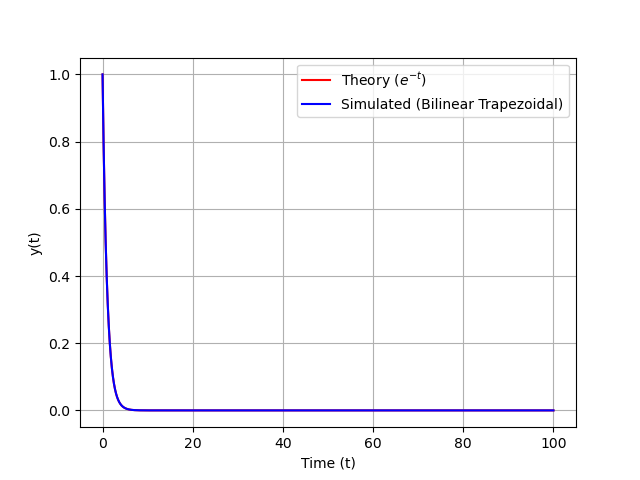
\includegraphics[width=1\linewidth]{figs/fig.png}
   \caption{Comparison between the Theoretical solution and Computational solution}
   \label{stemplot}
\end{figure}
\end{document}
